\documentclass[a4paper, 11pt]{article}

\usepackage[utf8]{inputenc}
\usepackage{amsmath,amssymb}
\usepackage{epsfig}  
\usepackage{setspace}
\usepackage{graphicx}

\voffset -0cm
\hoffset 0.0cm
\textheight 22cm
\textwidth 16cm
\topmargin 0.0cm
\oddsidemargin 0.0cm
\evensidemargin 0.0cm


\title{\bf{TP5 \\ Connected Component Applications}}
\author{}
\date{}


%%%%%%%%%%%%%%%%%%%%%%%%%%%
%%% Debut du document %%%%%
%%%%%%%%%%%%%%%%%%%%%%%%%%%
\begin{document}
\maketitle

\section*{\bf Counting blobs}

The goal here is to count the number of blobs in the image blobs.pgm using the connected component algorithm viewed in TP4.
Once you can identify each blob, compute their respective centroid and their volume (simply count the number of pixels inside each connected component).

\paragraph{Question} If we suppose that a blob is an ellipse, can you compute its major and minor axis ?

\begin{figure}
  \centering
  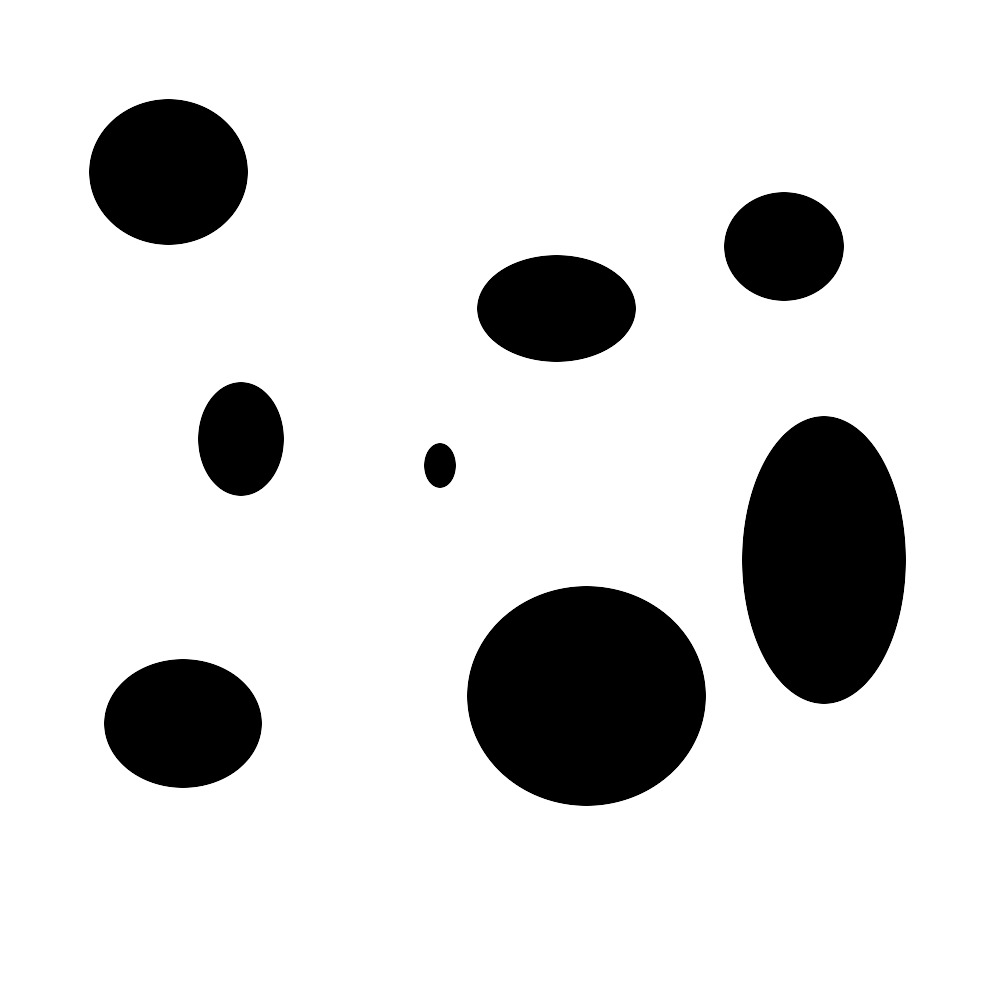
\includegraphics[width=0.5\textwidth]{blobs}
  \caption{An example of blobs}
\end{figure}

\section*{\bf Morphologic Dilatation and Erosion}

Morphology is a broad set of image processing operations that process images based on shapes. 
Morphological operations apply a structuring element to an input image, creating an output image of the same size. 
In a morphological operation, the value of each pixel in the output image is based on a comparison of the corresponding pixel in the input image with its neighbors. 

The most basic morphological operations are dilation and erosion. 
For each pixels $p$ in the input image, its value after dilation (resp. erosion) is the maximum (resp. minimum) value between all neighbor pixels defined by the mask.
More formally, let $P(p)$ be the value of the pixel $p$ in the input image. The dilation by a mask $\sigma$ denoted $P^{(\sigma)}$ of the input image is:
\[
  P^{(\sigma)}(p) = \max_{q\in\sigma(p)} P(q)
\]
and the erosion $P_{(\sigma)}$ is
\[
  P_{(\sigma)}(p) = \min_{q\in\sigma(p)} P(q).
\]

\paragraph{Question} Implement the two operations and test them using different masks (a line, a circl or a square for example).

\paragraph{Question} Use an operation of erosion to disconnect blobs in blobs2.pgm and then apply your connected component algorithm to count them.

\section*{\bf Morphological Opening}

Opening and closing are two important operators from mathematical morphology. 
They are both derived from the fundamental operations of erosion and dilation. 
Like those operators they are normally applied to binary images, although there are also graylevel versions. 
The basic effect of an opening is somewhat like erosion in that it tends to remove some of the foreground (bright) pixels from the edges of regions of foreground pixels. 
However it is less destructive than erosion in general. As with other morphological operators, the exact operation is determined by a structuring element. 
The effect of the operator is to preserve foreground regions that have a similar shape to this structuring element, or that can completely contain the structuring element, 
while eliminating all other regions of foreground pixels.

An opening is defined as an erosion followed by a dilation using the same structuring element for both operations.
The opening operator therefore requires two inputs: an image to be opened, and a structuring element.

\paragraph{Question} Use the opening operation to remove lines in art3.pgm (try different masks and see the results)

\paragraph{Question} Use the opening operation to isolate the big cells in cel4.pgm and then count them.

\end{document}

